\documentclass[tikz,border=4.14cm,a4paper]{standalone}
\usepackage{enumitem}
\usetikzlibrary{shapes.symbols,matrix,patterns}
\begin{document}
\pagenumbering{gobble}
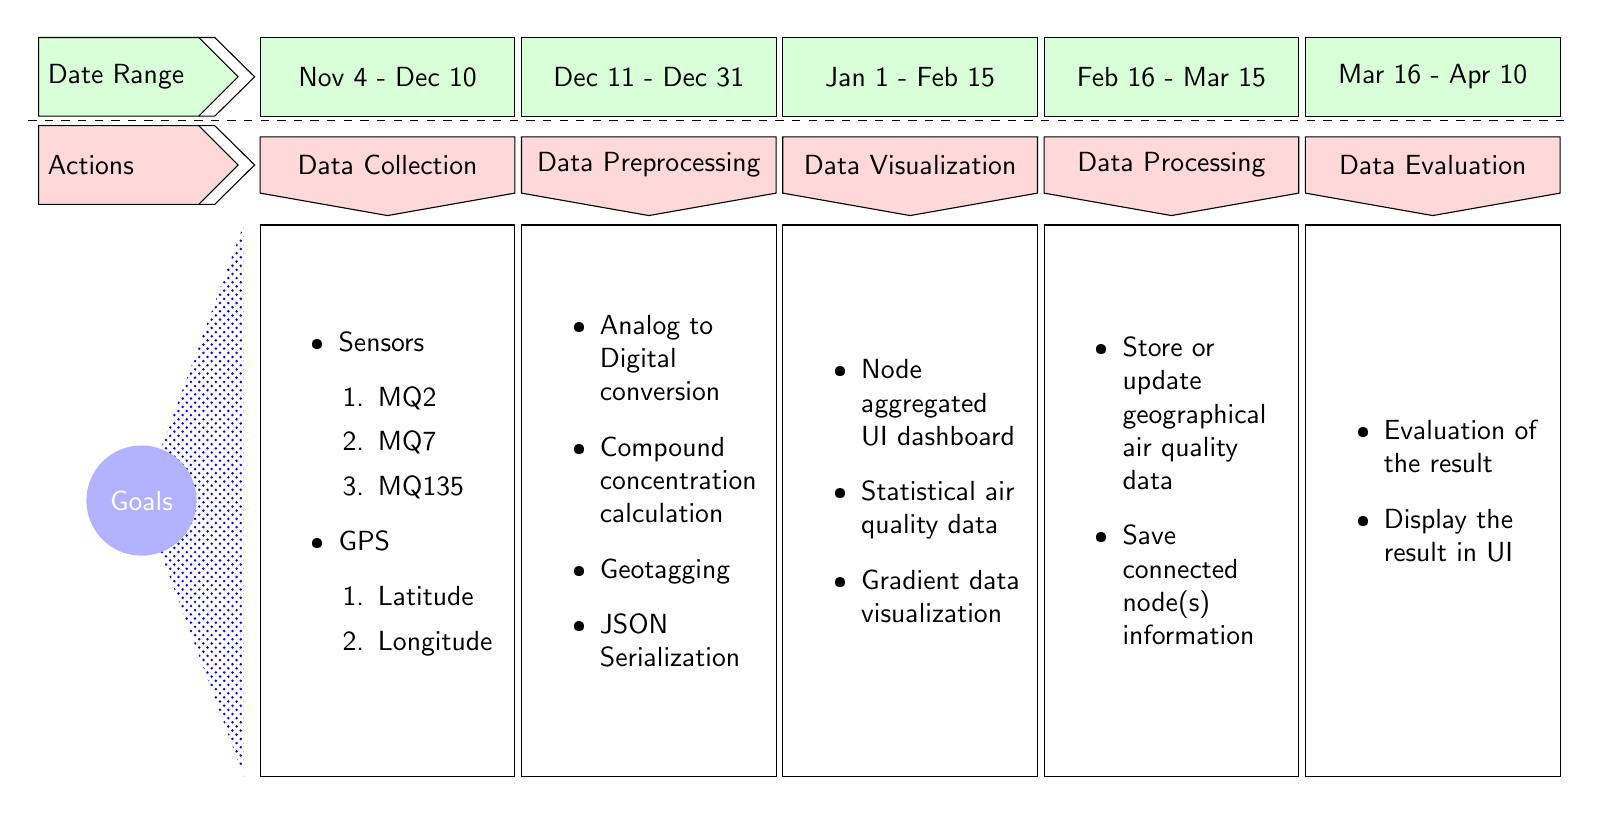
\begin{tikzpicture}[font=\sffamily,
box/.style={draw,fill=green!15,align=center},
arr/.style={draw,fill=red!15,signal, signal to=south, signal pointer angle=160,
align=center}, % Torjorn
tbox/.style={draw,align=left,minimum height=7cm},
sr/.style={signal,text width=1.8cm,align=left,alias=tmp,
append after command={(tmp.north east) -- ++ (0.2,0) -- ++(0.5,-0.5)
-- ++ (-0.5,-0.5) -- (tmp.south east)},draw=black}
]
 \matrix (mat) [matrix of nodes,column sep=2pt,row sep=3pt,nodes={text width=3cm,anchor=center,minimum height=1cm}]
 { |[sr,fill=green!15]| {Date Range} &
  |[box]| Nov 4 - Dec 10 & |[box]| Dec 11 - Dec 31 &
   |[box]| Jan 1 - Feb 15 &  |[box]| Feb 16 - Mar 15 &
  |[box]| Mar 16 - Apr 10  \\
 |[sr,fill=red!15]| {Actions} &
  |[arr]| Data Collection & |[arr]| Data Preprocessing &
  |[arr]| Data Visualization &  |[arr]| Data Processing &
  |[arr]| Data Evaluation \\
  & |[tbox]| {\begin{itemize}
   \item Sensors
   \begin{enumerate}[leftmargin=0.5cm]
       \item MQ2
       \item MQ7
       \item MQ135
   \end{enumerate}
   \item GPS
   \begin{enumerate}[leftmargin=0.5cm]
       \item Latitude
       \item Longitude
   \end{enumerate}

   \end{itemize}
   ~}
  & |[tbox]| {\begin{itemize}
   \item Analog to Digital conversion
   \item Compound concentration calculation
   \item Geotagging
   \item JSON Serialization
   \end{itemize}
   ~}
  & |[tbox]| {\begin{itemize}
   \item Node aggregated \\ UI dashboard
   \item Statistical air quality data
   \item Gradient data visualization
   \end{itemize}
   ~}
  & |[tbox]| {\begin{itemize}
   \item Store or update geographical air quality data
   \item Save connected node(s) information
   \end{itemize}
   ~}
    & |[tbox]| {\begin{itemize}
   \item Evaluation of the result
   \item Display the result in UI

   \end{itemize}
   ~}

   \\
 };
 \foreach \X in {1,2}
 {\draw ([yshift=-\pgflinewidth/2]mat-\X-1.north east) -- ++ (0.2,0) 
 -- ([xshift=2mm]mat-\X-1.east)
 -- ([xshift=2mm,yshift=\pgflinewidth/2]mat-\X-1.south east) -- ([yshift=\pgflinewidth/2]mat-\X-1.south east);
 }
 \path[pattern=crosshatch dots,pattern color=blue]
 ([xshift=-2mm]mat-3-2.north west) --
 ([xshift=-1.5cm]mat-3-2.west)
 node[circle,fill=blue!30,text=white,minimum size=1.4cm,align=center] {Goals}
 -- ([xshift=-2mm]mat-3-2.south west) -- cycle;
 \path (mat-1-1.south) -- (mat-2-1.north) coordinate[midway] (aux);
 \draw[dashed] (mat.west |- aux) -- (mat.east |- aux);
\end{tikzpicture}
\end{document}